\begin{figure}[h!]
	\centering
	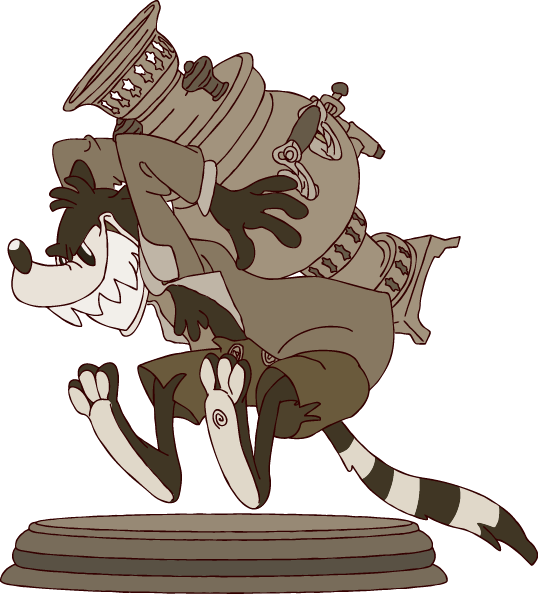
\includegraphics[width=0.4\linewidth, keepaspectratio]{tea_thief.png}
\end{figure}

В одном далеком лагере, в одной старой усадьбе, в самой дальней комнате жили два друга, два веселых и смелых парня~---~Влад и Влуд. 
Правила лагеря были очень строгими и большинство детей боялись сделать хоть шаг без спроса взрослых, но не наши отчаянные парни. 
В один из дней ребята решили пошалить, но их поймали и лишили сонника в наказание. 
Но парни не стали унывать, а разработали план по добыче вкусняшек. 
Они знали, что на первом этаже хранились огромные запасы чая, сладостей и различной вредной, но очень вкусной еды, и без присмотра она оставалась только ночью. 
Но вот незадача, ночью весь свет в усадьбе отключался, и коридоры патрулировались неспящими вожатыми, а иногда и самой Той-кого-нельзя-называть.  
Несколько ночей они следили за расписанием патрулей, а днем  пытались выяснить расположение вкусняшек, чтобы ночью в темноте иметь возможность обнаружить нужные за доли секунд.
И вот после всех приготовлений, в одну из самых темных и ненастных ночей, они решились на свою миссию. 
Для ее успеха, им было нужно сделать последнюю вещь~---~а именно выяснить, где добыть чай. 
Ребята выяснили, что для защиты от нерадивых, как они, воров, в коробке с чаем чайные пакетики хранились особым образом~---~на местах, чьи индексы являлись простыми числами лежал чай, 
а все остальные пакетики были обманками с сильным снотворным. 
Так как ребята были смышленые, они обратились к вам, чтобы вы за небольшой процент от добычи, написали им программу, которая поможет не ошибиться чаем.

\InputFile
\noindent

На первой строке передается количество чайных пакетов $K (2 \leq K \leq 200)$.
На следующей строке передаются веса чайных пакетиков ($0 \leq x_i \leq 100$).


\OutputFile
\noindent

Вывести количество безопасных пакетиков.

\SAMPLES